\documentclass[12pt]{article}
\usepackage[hidelinks]{hyperref}    
\usepackage[all]{hypcap}   
\usepackage{graphicx}
\usepackage{amsmath}
\usepackage{listings}
\usepackage{xcolor}

% Define custom settings for HACK assembly language
\lstdefinelanguage
    [HACK]{Assembler}
    {morekeywords={@SP, @LCL, @ARG, @THIS, @THAT, @SCREEN, @KBD}, % Common HACK symbols
     alsoother={=,;,@},  % Symbols used in HACK assembly
     sensitive=true,     % Case-sensitive
     morecomment=[l]//,  % Define comments to start with "//"
    }

% Set up the listing style for HACK assembly
\lstset{
    language=[HACK]Assembler,
    basicstyle=\ttfamily\small,      % Small monospace font
    keywordstyle=\color{blue},       % Keywords in blue
    commentstyle=\color{gray},       % Comments in gray
    stringstyle=\color{red},         % Strings in red
    tabsize=4,
    showstringspaces=false,
    numbers=left,                    % Line numbers on the left
    numberstyle=\tiny\color{gray},
    breaklines=true,
    frame=single,                    % Frame around the code
}
\graphicspath{{../images/}}
\author{Andrea Malvezzi}
\title{\textbf{Architettura degli Elaboratori\\ ISA del processore HACK}}
\date{05 novembre, 2024}
\author{Andrea Malvezzi}
\begin{document}
\maketitle
\pagebreak
\tableofcontents
\pagebreak

\section{Che cos'è l'ISA}
\label{sec:whats_ISA}
L'ISA è l'interfaccia tra HW e SW.
Costituisce il set di istruzioni con cui opera la CPU e di conseguenza, varia di architettura in architettura.

\section{L'architettura HACK}
\label{sec:HACK_architecture}
L'architettura HACK non segue né la filosofia CISC né quella RISC e, data la sua semplicità, in essa ad ogni istruzione eseguita corrisponde un ciclo di clock.
Qui si usano una RAM (per contenere i dati di un programma in esecuzione) e una ROM (per contenere il programma \textit{stesso}) a 16 bit. \\
Si utilizzano prevalentemente tre registri di memoria: \textbf{A}, \textbf{D} ed \textbf{M}.
\\Il registro M è particolare, in quanto contiene il valore del registro di memoria RAM attualmente puntato da A. Questo si indica con RAM[A]. \\
Oltre a questi due si usa inoltre il \textbf{Program Counter}, o \textbf{PC}. In esso è contenuto l'indirizzo della prossima istruzione da eseguire e si indica con ROM[PC].

\section{Tipi di istruzione}
\label{sec:tipi_istruzione}
Esistono due tipi di istruzioni:
\begin{itemize}
    \item A-instruction: quelle che lavorano sulla memoria (che caricano valori in A);
    \item C-instruction: quelle che eseguono un instruzione (sfruttando l'ALU) prelevando gli operandi dai registri A,D ed M.
\end{itemize}
Le C-instruction solitamente seguono la forma generale $\text{dest} = \text{comp}; \text{jump}$, dove:
\begin{itemize}
    \item \textbf{dest}: opzionale. Specifica dove memorizzare il risultato\\dell'operazione;
    \item \textbf{comp}: specifica l'operazione da eseguire;
    \item \textbf{jump}: opzionale. Specifica se, dopo aver eseguito $\text{dest} = \text{comp}$ occorre fare un salto nel programma alla linea specificata dal valore del registro A (esegue $\text{PC} = A)$. Funziona effettivamente come un \textit{if} eseguito sempre rispetto allo zero. 
\end{itemize}

\subsection{Tutte le possibili operazioni}
\label{ssec:operazioni_possibili}
A seguire tutte le possibili operazioni eseguibili nell'architettura HACK.
\begin{figure}[!htb]
    \centering
    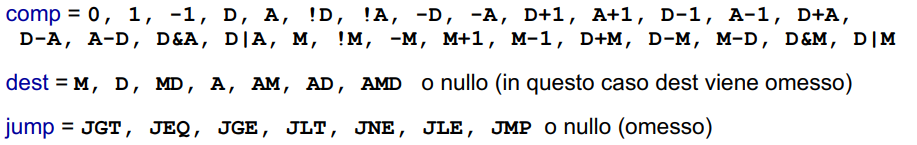
\includegraphics[width=.9\linewidth,height=.40\textheight,keepaspectratio]{ISA_HACK/operazioni.png} % essenzialmente resiza l'immagine
    \begin{center}
        \caption{\label{fig:operazioni} Se un'operazione che si desidera eseguire non compare qui, allora occorre cambiare approcio.} % label fuori da caption spesso non va, mettilo dentro
    \end{center}
\end{figure}
\subsubsection{Esempio di operazione}
\label{sssec:operazioni_esempi}
\begin{gather*}
    @2\\
    \text{D}=\text{D} + 1;\text{JLT}
\end{gather*}
Questa riga di codice aumenta di 1 il valore del registro D, poi controlla che questo valore sia strettamente minore di 0.
Nel caso in cui questa condizione risultasse verificata, verrà effettuato un JUMP alla riga corrispondente al valore corrente di A, quindi, alla seconda.

\section{Le etichette}
\label{sec:etichette}
Un'etichetta è un'istruzione composta di due parti: quella di dichiarazione e quella di chiamata.

\subsection{Dichiarazione di etichetta}
\label{ssec:dichiarazione_etichetta}
Un'etichetta fornisce un modo per non dover scrivere a mano (e quindi commettere errori) ogni A-instruction prima di effettuare un salto.
Difatti, l'etichetta prende il valore del numero di riga in cui viene dichiarata, permettendo poi di saltare a quella eventuale riga qualora risultasse necessario.
\subsubsection{Esempio di dichiarazione di etichetta}
\label{sssec:esempio_dichiarazione_etichetta}
\begin{gather*}
    (\text{MIA\_ETICHETTA})\\
    \dots \text{codice} \dots
\end{gather*}
Qui l'etichetta viene definita prima di un blocco di codice e prende il nome di MIA\_ETICHETTA.
Questa etichetta avrà quindi ora il valore della riga a cui è stata dichiarata (quella prima del blocco di codice).

\subsection{Utilizzo dell'etichetta}
\label{ssec:utilizzo_etichetta}
Questa etichetta contiene ora il numero della riga in cui è stata dichiarata e, in quanto tale, fornisce un modo per saltare a tale riga mediante una istruzione JUMP.
\subsubsection{Esempio di utilizzo dell'etichetta}
\label{sssec:esempio_utilizzo_etichetta}
\begin{gather*}
    @\text{MIA\_ETICHETTA}\\
    0;\text{JMP}
\end{gather*}
Questo ci permette di assegnare ad A il valore della riga in cui l'etichetta è stata dichiarata, per poi eseguire un salto incondizionato (0 è sempre zero, quindi il JMP verrà sempre effettuato) alla riga corrispondente all'inizio del blocco di codice sottostante all'etichetta.
\pagebreak

\section{Costrutti della programmazione}
\label{sec:costrutti_programmazione}

\subsection{If-then-else}
\label{ssec:if_then_else}
Si può ricreare il costrutto if-then-else tramite JUMP, A/C-instruction ed etichette.
\begin{lstlisting}
    // Costrutto if-then-else
    D=1             // Dato da testare

    @CASE_FALSE     // A=riga del caso false
    D;JLE           // Se D <= 0, JUMP al valore di A

    // Se salto, questo blocco non viene eseguito
    ...caso true... 

    @END            // A=riga fine codice
    0;JMP           // Salto incondizionato

    (CASE_FALSE)    // Dichiaro l'etichetta
    ...caso false...

    (END)           // Dichiaro l'etichetta
    ...fine codice...
\end{lstlisting}

\pagebreak
\subsection{Ciclo while}
\label{ssec:while}
Anche il ciclo while si può ricreare mediante JUMP, A/C-instruction ed etichette, seppure in maniera leggermente più complessa.
\begin{lstlisting}
    // Ciclo while
    D=10             // Variabile per iterazione

    (LOOP)          // Dichiaro inizio loop
    D; JLE          // JMP se D<=0
    
    ...codice...    // Se salto, questo viene saltato

    @LOOP           // Al termine del codice, rifai
    0;JMP           // Salto incondizionato

    (EXIT)          // Dichiaro uscita loop
    ...altro codice...
\end{lstlisting}

\pagebreak
\section{Cose a cui prestare attenzione}
\label{sec:nb_1}

\subsection{Fine dei programmi}
\label{ssec:fine_programma}
Di base i programmi non finiscono, ma continuano ad incrementare il PC fino a che non si esaurisce la ROM.
Per evitare questa behaviour, è buona pratica terminare un programma con un ciclo dummy che previene quindi di andare ad eseguire istruzioni scritte nelle celle della ROM successive.
\begin{lstlisting}
    // Ciclo dummy
    ...codice programma...
    
    // Dichiaro un ciclo infinito
    (END)       // Dichiaro fine programma
        @END    // A=Riga precedente
        0;JMP   // Salto incondizionato
\end{lstlisting}

\subsection{Comparazioni tra valori diversi da 0}
\label{ssec:compare_values}
Come visto in precedenza, esistono solo comparazioni rispetto lo 0. Per ovviare a questa limitazione, si possono usare la somma e la sottrazione.
\begin{lstlisting}
    // A <= 10?
    @2      // A=2
    D=10    // D=10
    D=D-A   // D=D-A, quindi D=10-2

    @ELSE   // Preparo A per saltare all'else case
    D:JLE   // Se D<=0, JUMP

    ...caso true...
    @END    // Termina programma
    0;JMP   // Salto incondizionato

    (ELSE)  // Dichiaro else case
        ...caso false...

    (END)   // Dichiaro ciclo dummy finale
        @END
        0;JMP
\end{lstlisting}

\section{Le variabili}
\label{sec:variables}
Anche in asm HACK si hanno le variabili, anche se funzionano in modo leggermente diverso.
Qui si definiscono come A-instruction e si va a modificare il valore interno al loro registro.
\begin{lstlisting}
    // Esempio di uso delle variabili
    @i          // Variabile i
    M=1         // Registro di i pari ad 1 (RAM[i]=1)

    (LOOP)      // Dichiaro inizio loop
        @i      // uso i
        D=M     // D=Valore registro di i
        @10     // A=10
        D=D-A   // D=D-A, quindi D=i-10

        @END    // Preparo a terminare il programma
        D;JGT   // Se D>0, JUMP

        ...codice loop...
        @i      // Uso i
        M=M+1   // Aumento di 1 il valore di RAM[i]
        ...codice loop...

        @LOOP   // Preparo per ricominciare
        0;JMP   // Salto incondizionato
    
        (END)   // Dichiaro ciclo dummy finale
            @END
            0;JMP
        
        // La variabile i serve ad iterare nel loop
        // fino a quando non equivale ad 11 (i-10>10)
\end{lstlisting}
Esistono inoltre variabili pre-definite per accedere in maniera più esplicita alla memoria RAM, come @R\textit{n}, dove \textit{n} va da 0 a 15. 
\pagebreak
\section{Cose a cui prestare attenzione}
\label{sec:nb_2}

\subsection{Naming conventions}
\label{ssec:nb_naming_conventions}
Generalmente le variabili hanno nomi in minuscolo, mentre le etichette in maiuscolo.

\subsection{Nota sull'uso delle variabili}
\label{ssec:nb_using_variables}
In termini pratici, i primi 16 indirizzi della memoria RAM (da @R0 a @R15) sono riservati per l'esecuzione del programma in esecuzione.
Tutti gli indirizzi successivi saranno utilizzati da eventuali variabili, a scelta dell'assemblatore. \\
Per questo motivo, qualora in un programma ci si ritrovasse a dover scrivere qualcosa come @16 oppure un qualunque valore superiore a 15, allora non si dovranno utilizzare variabili, in quanto queste rischierebbero di essere sovrascritte.

\pagebreak
\section{Esercizi}
\label{sec:exercises}

\subsection{Esercizi introduttivi}
\label{ssec:beginner_friendly}

\subsubsection{D=0}
\begin{lstlisting}
    D=0
\end{lstlisting}

\subsubsection{A=1 e D=1}
\begin{lstlisting}
    // Con due istruzioni separate:
    @0      // A=0
    D=0     // D=0. Anche D=A andrebbe bene

    // Con la scrittura compatta:
    AD=0    // Assegno CONTEMPORANEAMENTE A e D a 0
\end{lstlisting}

\subsubsection{D=3}
\begin{lstlisting}
    // Non esiste l'istruzione D=n con n diverso da 1
    @3  // Prima assegno ad A il valore di 3

    D=A // Poi assegno a D il valore di A
\end{lstlisting}

\subsubsection{D=RAM[3]+3}
\begin{lstlisting}
    @3      // Assegno ad A valore pari a 3
    D=M     // D=RAM[3]
    D=D+A   // D=D+A, quindi D=RAM[3]+3
\end{lstlisting}

\subsubsection{D=3+4}
\begin{lstlisting}
    @3      // A=3
    D=A     // D=A, quindi D=3
    @4      // A=4
    D=D+A   // D=D+A, quindi D=3+4
\end{lstlisting}

\subsubsection{RAM[3]=7}
\begin{lstlisting}
    @7      // A=7
    D=A     // D=7
    @3      // A=3
    M=D     // RAM[3]=7
\end{lstlisting}

\subsubsection{D=RAM[A]+3}
\begin{lstlisting}
    D=M     // Supponendo che A sia dichiarata a priori
    @3      // A=3
    D=D+A   // D=D+A, quindi D=RAM[A]+3
\end{lstlisting}

\subsection{Esercizi significativi}

\subsubsection{D=D-3}
\begin{lstlisting}
    @3      // A=3
    D=D-A   // Supponendo che D sia dichiarata a priori
\end{lstlisting}

\subsubsection{D=10-RAM[5]}
\begin{lstlisting}
    @10     // A=10
    D=A     // D=A, quindi D=10
    @5      // A=5
    D=D-M   // D=D-M, quindi D=10-RAM[5]
\end{lstlisting}

\subsubsection{RAM[0]=RAM[0]+2}
\begin{lstlisting}
    @2      // A=2
    D=A     // D=A, quindi D=2
    @0      // A=0
    M=M+D   // M=M+D, quindi RAM[0]=RAM[0]+2
\end{lstlisting}

\subsubsection{RAM[RAM[0]]=RAM[0]}
\begin{lstlisting}
    @0      // A=0
    AD=M    // A e D = M, quindi A e D = RAM[0]
    M=D     // M=D, quindi RAM[RAM[0]]=RAM[0]
    // M equivale a RAM[RAM[0]] in quanto A=RAM[0]
\end{lstlisting}

\subsubsection{RAM[2]=RAM[0]+RAM[1]}
\begin{lstlisting}
    @0      // A=0
    D=M     // D=RAM[0]
    @1      // A=1
    D=D+M   // D=RAM[0]+RAM[1]
    @2      // A=2
    M=D     // M=D, quindi RAM[2]=RAM[0]+RAM[1]
    // Nessuno vieta di spezzettare il problema!
\end{lstlisting}

\subsection{Esercizi con salti}

\subsubsection{Se RAM[0]\textgreater 0, JUMP all'indirizzo in RAM[1]}
\begin{lstlisting}
    @0      // A=0
    D=M     // D=RAM[0]
    @1      // A=1
    A=M     // A=RAM[1]
    D;JGT   // Se RAM[0]>0, JUMP a RAM[1]
\end{lstlisting}

\subsubsection{D=D+1, poi se D=0 JUMP a istruzione 3}
\begin{lstlisting}
    D=D+1   // Incrementa D
    @3      // A=3
    D;JEQ   // Se D=0, JUMP a valore di A (quindi 3)
\end{lstlisting}

\pagebreak
\subsubsection{RAM[0]=RAM[5] e se RAM[5]\textless\textgreater 0 JUMP a istruzione 3}
\begin{lstlisting}
    @5      // A=5
    D=M     // D=RAM[5]
    @0      // A=0
    M=D     // RAM[0]=RAM[5]
    @3      // A=3
    D;JNE   // Se RAM[5] != 0, JUMP a valore di A
\end{lstlisting}

\subsection{Esercizi con le etichette}

\subsubsection{Implementazione moltiplicazione}
\begin{lstlisting}
    // Volendo eseguire RAM[2] = RAM[0] * RAM[1]:
    @2          // A=2
    M=0         // RAM[2]=0
    @4          // A=4
    M=1         // RAM[4]=1, contatore per loop

    (LOOP)      // Inizio loop
        @4      // A=4
        D=M     // D=RAM[4], prendo contatore
        @1      // A=1 
        D=D-M   // RAM[4]=RAM[4]-RAM[1]
        
        @END    // Preparo a terminare
        D;JGT   // Se contatore-RAM[1]>0, termina

        @0      // A=0
        D=M     // D=RAM[0], val da moltiplicare
        @2      // A=2
        M=M+D   // sommo RAM[0] a RAM[2]

        @LOOP   // Preparo a rifare
        0;JMP   // Salto incondizionato
    
    (END)       // Ciclo dummy finale
        @END
        0;JMP
\end{lstlisting}

\subsubsection{Implementazione moltiplicazione senza quarto registro}
\begin{lstlisting}
    // Volendo eseguire RAM[2] = RAM[0] * RAM[1]:
    @2          // A=2
    M=0         // RAM[2]=0
    
    (LOOP)      // Inizio loop
        @0      // A=0
        D=M     // D=RAM[0], val da moltiplicare
        @2      // A=2
        M=M+D   // sommo RAM[0] a RAM[2]

        @1
        DM=M-1
        @LOOP
        D;JGT   // Rifai se RAM[1]-1>0
    
    ...resto codice...
\end{lstlisting}

\subsubsection{RAM[10]=max(RAM[9..0])}
\begin{lstlisting}
    @9      // A=9
    D=A     // D=9
    @11     // A=11
    M=D     // RAM[11]=9, contatore
    @9      // A=9
    D=M     // D=RAM[9], il primo valore equivale a max
    @10     // A=10
    M=D     // RAM[10]=RAM[9]
        
    (LOOP)          // Dichiaro inizio loop
        @11     // A=11
        D=M     // D=RAM[11], contatore
        @END    // Preparo a terminare
        D;JEQ   // Se D equivale a 0, JUMP

        @11     // Rimetto A=11
        M=M-1   // RAM[11]--
        A=M     // A=RAM[11]
        D=M     // D=RAM[A]
        @10
        D=M-D   // D=(Max)-(valore corrente)
        @SET    // Preparo a cambiare max
        D;JLT   // Se D<0, JUMP

        @LOOP   // Preparo a rifare
        0;JMP   // Salto incondizionato   

    (SET)
        @11     // A=11
        D=M     // D=RAM[11], contatore
        A=D     // A=contatore
        D=M     // D=(valore corrente)
        @10     // A=10
        M=D     // Cambio max
        
        @LOOP   // Preparo a rientrare nel loop
        0;JMP   // Salto incondizionato

    (END)       // Ciclo dummy finale
        @END
        0;JMP
\end{lstlisting}
Di questo esercizio si trova una copia del codice eseguibile nell'emulatore nella cartella \_esercizi.

\end{document}